\section{Equazione di D'Alembert}
\lecture{5}{12 marzo 2024}

Oggi cerchiamo le soluzioni dell'equazione di D'Alembert. È un'equazione molto generale valida per le onde: meccanica, acustica, fluidodinamica, ottica, elettromagnetismo ecc. Si ottiene nel caso \textbf{delle piccole oscillazioni}.

\begin{gather*}
	\frac{\partial ^{2} \xi }{\partial x^{2} } = \frac{1}{v^{2} }\frac{\partial ^{2} \xi }{\partial t ^{2} }\\
	\hat{L} = \left(\frac{\partial ^{2} }{\partial x^{2} } - \frac{1}{v^{2} }\frac{\partial ^{2} }{\partial t ^{2} }\right) 
\end{gather*}

\(\hat{L} \) è un operatore lineare, quindi vale il principio di sovrapposizione. È un'equazione omogenea, quindi è sempre presente la soluzione banale. È un'equazione alle derivate seconde, quindi per ogni punto dell'asse x è necessario specificare due condizioni iniziali (nell'oscillatore armonico ci bastavano due condizioni iniziali, il punto era solo uno!).

\[
	\begin{cases}
		\xi (x, t_0) = f(x)
		\dot{\xi } (x, t_0) = g(x) 
	\end{cases}	
\]

Si nota che particolari combinazioni delle variabili spazio e tempo conducono a considerare soluzioni unidimensionali: \(s=x-vt\) \(w=x+vt\). Dimostriamolo.

\begin{gather*}
	\xi (x,t) = f(s) = f(x-vt) \text{ con } s(x,t)=x-vt\\
	\frac{\partial \xi }{\partial x} = \frac{\partial f}{\partial x} = \frac{\partial f}{\partial x} \frac{\partial s}{\partial x} = \frac{\mathrm{d}f}{\mathrm{d}s} = f^{\prime} \\
	\rightsquigarrow \frac{\partial \xi ^{2} }{\partial x^{2} } = \frac{\partial f^{\prime} }{\partial x} = \frac{\partial f^{\prime} }{\partial s} \frac{\partial s}{\partial x} = \frac{\mathrm{d}f^{\prime} }{\mathrm{d}s} = f^{\prime\prime} \\
	\frac{\partial \xi }{\partial t} = \frac{\partial f}{\partial t} = \frac{\partial f}{\partial s} \frac{\partial s}{\partial t} = -v \frac{\mathrm{d}f}{\mathrm{d}s} = - v f^{\prime} \\
	\rightsquigarrow \frac{\partial \xi ^{2} }{\partial t^{2} } = -v \frac{\partial f^{\prime} }{\partial t}  = - v \frac{\partial f^{\prime} }{\partial s} \frac{\partial s}{\partial t} = v ^{2} f^{\prime\prime} 
\end{gather*}

Ottengo quindi l'equazione di D'Alembert nella forma \(f^{\prime\prime} = \frac{1}{v^{2} } v ^{2} f^{\prime\prime} \), che è verificata \(\forall f\). È sufficiente che sia derivabile due volte. Si può dimostrare allo stesso modo che \(\xi (x,t) = g(x+vt)\) è sempre una soluzione. Siamo passati dal cercare funzioni in due variabili al cercare soluzioni in una variabile.

\begin{gather*}
	\xi (x,t) = f(s) + g(w) = f(x-vt) + g(x+vt) \text{ è soluzione } \forall f,g \in \mathcal{C} ^{2}  \\
	\begin{cases}
		\xi (x,t) = f(x-vt) &\text{ è detta onda progressiva}\\
		\xi (x,t) = g(x+vt) &\text{ è detta onda regressiva} 
	\end{cases}
\end{gather*}

\subsection{Onda progressiva}

Studiamo un'onda impulsiva progressiva di forma gaussiana: \(\xi (x,t) = f(s) = A e^{- \alpha (x-vt)^{2} }\). Rappresentiamo la funzione per \(t_0=0\) (o equivalentemente in funzione di s). In questo caso ha un massimo in \(s_0 = x_0 = 0\).
\begin{figure}[H]
	\centering
	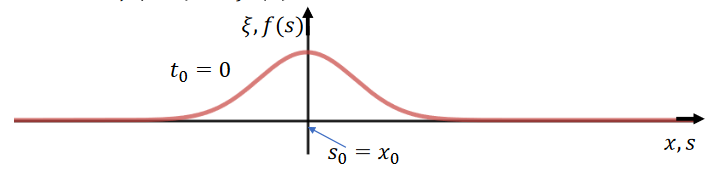
\includegraphics[width=0.8\textwidth]{screenshots/2024-03-12-11-47-01.png}
\end{figure}
Se guardo l'onda in un istante di tempo successivo l'onda si è spostata verso destra:
\begin{figure}[H]
	\centering
	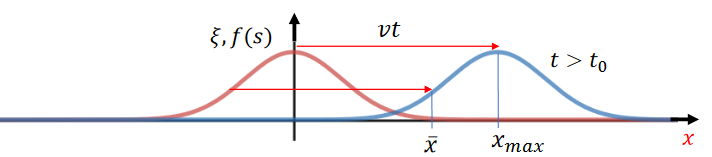
\includegraphics[width=0.8\textwidth]{screenshots/2024-03-12-11-48-57.png}
\end{figure}
Il massimo si può trovare sempre ponendo \(s=0 \rightsquigarrow x_{max} - vt = 0 \rightsquigarrow x_{max} = vt  \). Il massimo si propaga con un'equazione lineare! Non accelera. La forma dell'onda non varia, quindi ogni punto della curva si sposta verso destra con velocità \(v\): \(s = \overline{s} \rightsquigarrow x-vt = \overline{s} \rightsquigarrow \overline{x} = \overline{s} + vt \). Queste considerazioni valgono per qualsiasi onda progressiva.

Le onde meccaniche si descrivono sempre nel sistema di riferimento S in cui il mezzo è fermo (è un SdR privilegiato). Se mi muovo in un sistema di riferimento S' con velocità \(v\) verso destra la funzione \(\xi \) non dipende più dal tempo: l'onda appare ferma. Tuttavia non risolve più l'equazione di D'Alembert (non compaiono derivate seconde rispetto al tempo)! Per studiare le onde devo fare attenzione al sistema di riferimento e pormi in quello privilegiato.

\subsection{Velocità di un'onda}

Il parametro \(v = \sqrt{\frac{T}{\mu }} \) rappresenta quindi la velocità apparente di ogni punto dell'onda. Su corde leggere e sottili (\(\mu \) piccolo) le velocità sono grandi. Su corde grandi e spesse (\(\mu \) grande) le velocità sono piccole. Maggiore è la tensione, maggiore è la velocità.

\subsection{Sovrapposizione di onde}

Le onde possono urtarsi, ma la loro forma non cambia. Facciamo l'esempio di un'onda regressiva e una progressiva:
\begin{figure}[H]
	\centering
	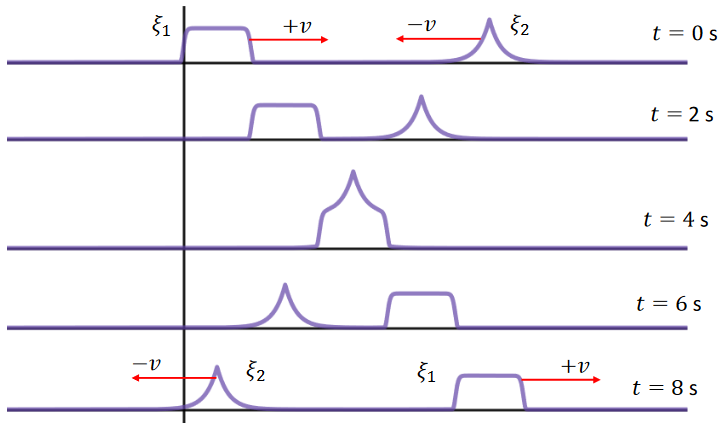
\includegraphics[width=0.6\textwidth]{screenshots/2024-03-12-12-02-37.png}
\end{figure}